\section{Impicit ODE solver}
Considering again the \textit{Initial Value Problem}.
$$
\frac{d}{d t} x(t)= \dot{x}(t)=f(t, x(t), p), \quad x\left(t_{0}\right)=x_{0},
$$
where $x \in \mathbb{R}^{n_{x}}$ and $p \in \mathbb{R}^{n_{p}}$. In the following equations the parameters p are implicit in $f(t, x(t)) = f(t, x(t), p)$.

\subsection{Implicit Euler}
Whereas the Explicit Euler intuitively takes a discrete step forward with $\dot{x}_k$, the Implicit Euler intuitively takes a step \textit{backward} with $\dot{x}_{k+1}$ in each iteration \textit{k} \cite{JrgensenScientificEquationsb}:

\begin{equation}
    x_{k+1}=x_{k}+\Delta t_k f\left(t_{k+1}, x_{k+1}\right)
\end{equation}

Where $\Delta t_k$ is the step size in iteration \textit{k}. It discretises the continuous ODE in the same fashion as the Explicit Euler. The method is analogous to taking the tangent in $x(t_{k+1}) = x_{k+1}$ and taking a $\Delta t_k$ step along the tangent:

\begin{equation}
\frac{x\left(t_{k+1}\right)-x\left(t_{k}\right)}{\Delta t_{k}} \approx \frac{d}{d t} x\left(t_{k+1}\right)=f\left(t_{k+1}, x\left(t_{k+1}\right)\right)
\end{equation}

One natural hurdle arises: We don't know the $\dot{x}_{k+1} = f\left(t_{k+1}, x\left(t_{k+1}\right)\right) = f\left(t_{k+1}, x_{k+1}\right)$ because $x_{k+1}$ is unknown (it is the one we wish to calculate in iteration \textit{k}). Solution: Estimate it using \textit{Newton's method}.

\\\

\textbf{Newton's Method} \\
Newton's method finds the root of a residual function $R(x_{k+1})=0$ using a 1st order Taylor expansion at $x_{k+1}$:
\begin{equation}
    R(x_{k+1}) \approx R(x_k) + \frac{\partial R}{\partial x}\left(x_{k
    }\right)\left(x_{k+1} - x_{k}\right)
\end{equation}

Which can be solved as a linear system of equations \cite{JrgensenScientificEquationsb}. So by formulating the Implicit Euler problem as a residual function: 

\begin{equation}
R\left(x_{k+1}\right)=x_{k+1}-\Delta t f\left(t_{k+1}, x_{k+1}\right)-x_{k}=0
\end{equation}

One can implicitly estimate $x_{k+1}$ by minimising the residual function. In practice, one chooses a tolerance $\epsilon$ for criteria of convergence where $\|R(x)\|_{\infty} \leq \epsilon$ or if a maximum number of iterations has been reached. Using the linear systems formulation, the function is then minimised by Newton's Method by iterating over

$$
\begin{aligned}
&M \Delta x_{k+1}=R\left(x_{k+1}^{[l]}\right) \\
&x_{k+1}^{[l+1]}=x_{k+1}^{[l]}-\Delta x
\end{aligned}
$$

in each iteration \textit{l} where $M=\frac{\partial R}{\partial x}\left(x_{k+1}\right)$ [ibid.]. A decent initial guess at $l=0$ is the simple Explicit Euler step:

$$
x_{k+1}^{[0]}=x_{k}+\Delta t_k f\left(t_{k}, x_{k}\right)
$$

\\\

As with the Explicit Euler, a question arises on choosing an appropriate step size $\Delta t_k$. This gives rise to Implicit Euler with fixed step size:

\begin{equation*}
    \Delta t_k = \Delta t = h \quad \forall_k
\end{equation*}

or Implicit Euler with adaptive step size where $\Delta t_k$ changes in each iteration k. The ladder approach is discussed in further detail in Section 3.3.













\subsection{MATLAB implementation fixed step size}
See the following MATLAB implementation of the Implicit Euler with fixed step size (as described in Section 3.1), well-suited for non-stiff problems.

\begin{adjustwidth*}{0cm}{-0.4cm}
\begin{lstlisting}[frame=single, language=Matlab,caption=Implicit Euler (fixed step size), label=ImplicittEulerFixie]
function [T,X] = ImplicitEulerFixedStepSize(funJac,ta,tb,N,xa,varargin)
    % Compute step size and allocate memory
    dt = (tb-ta)/N;
    nx = size(xa,1);
    X = zeros(nx,N+1);
    T = zeros(1,N+1);

    tol = 1.0e-8;
    maxit = 100;
    % Eulers Implicit Method
    T(:,1) = ta;
    X(:,1) = xa;
    for k=1:N
        [f, J] = feval(funJac,T(k),X(:,k),varargin{:}); T(:,k+1) = T(:,k) + dt;
        xinit = X(:,k) + f*dt;
        X(:,k+1) = NewtonsMethodODE(funJac,...
            T(:,k), X(:,k), dt, xinit, tol, maxit, varargin{:});
    end
    % Form a nice table for the result
    T=T';
    X=X';
end
\end{lstlisting}
\end{adjustwidth*}

Which utilises Newton's Method:

\begin{adjustwidth*}{0cm}{-0.4cm}
\begin{lstlisting}[frame=single, language=Matlab,caption=Newton's Method, label=Newton]
function x = NewtonsMethodODE(FunJac, tk, xk, dt, xinit, tol, maxit, varargin)
    k=0;
    t=tk+dt;
    x = xinit;
    [f,J] = feval(FunJac,t,x,varargin{:});
    R=x-f*dt-xk;
    I = eye(length(xk));
    while( (k < maxit) & (norm(R,'inf') > tol) )
        k=k+1;
        dRdx=I-J*dt;
        dx = dRdx\R;
        x=x-dx;
        [f,J] = feval(FunJac,t,x,varargin{:});
        R=x-dt*f-xk;
    end
end
\end{lstlisting}
\end{adjustwidth*}















\subsection{MATLAB implementation adaptive step size}
See the following MATLAB implementation of the Implicit Euler with adaptive step size, well-suited for stiff and non-stiff problems. The embedded error estimation is based on \textit{stop doubling}, i.e. estimating the error of a full step from the more accurate two half-steps. This procedure has been explained in full detail in Section \ref{sec:ExplicitEulerAdaptive}.

\begin{adjustwidth*}{0cm}{-0.4cm}
\begin{lstlisting}[frame=single, language=Matlab,caption=Implicit Euler (adaptive step size), label=ExplicitEulerFixie]
function [T,X,iter] = ImplicitEulerAdaptiveStep(...
    funJac,tspan,x0,h0,abstol,reltol,varargin)
epstol = 0.8;
facmin = 0.1;
facmax = 5.0;

t0 = tspan(1);
tf = tspan(2);

iter = 0;
% Initial condtions
t = t0;
h = h0; % = dt (step size - bliver modificeret)
x = x0;

% Output
T = t;
X = x';

% Newton syuff
tol = 1e-05;
maxit = 1000;

%% Main algorithm
while t < tf
    iter = iter +1;
    if (t + h >tf)
        h = tf-t;
    end
    f = feval(funJac,t,x,varargin{:});
    AcceptStep = false;
    while ~AcceptStep
        %Take step of size h
        xinit = x + h*f; % Gæt på x+1
        x1 = NewtonsMethodODE(funJac, t, x, h, xinit, tol, maxit, varargin{:});

        %Take step of size h/2
        hm = 0.5*h;
        xinitm = x + hm*f;
        tm = t + hm;

        xm = NewtonsMethodODE(funJac, tm, x, hm, xinitm, tol, maxit, varargin{:});
        
        xinitm2 = x + 2*hm*f ; % = xinit (og derfor redundant)
        x1hat = NewtonsMethodODE(funJac, tm, xm, hm, xinitm2, tol, maxit, varargin{:});

        % Error estimation
        e = x1hat-x1; % Estimate of global error
        r = max(abs(e) ./ max(abstol,abs(x1hat).*reltol));

        AcceptStep = (r <= 1.0);
        if AcceptStep
            t = t+h;
            x = x1hat;

            T = [T;t];
            X = [X;x'];
        end
        % Asymptotic step size controller
        h = max(facmin, min(sqrt(epstol/r), facmax))*h;
    end
end
\end{lstlisting}
\end{adjustwidth*}










\subsection{Van der Pol}


The phase potraits as obtained by solving the Van der Pol problem using the Adaptive Explicit Euler and Fixed (step size) Explicit Euler is seen in Figure \ref{fig:2_4a} and \ref{fig:2_4b}. The problem is solved for t = [0, 32] with $\mu = 3$ and $\mu =20$. Tolerances chosen are $reltol = abstol = \{10^{-2}, 10^{-4}, 10^{-6}\}$. Now a natural question arises, which fixed step sizes $h$ should be chosen for comparison with the adaptive method? The fixed step size $h$ was chosen to result in same number of steps as for the adaptive solution for comparison purposes.

\\
Clearly, for the stiff problem ($\mu = 20$) the fixed step size $h \approx 0.1$ is infeasible. The method is unstable and explodes towards $\infty$ (Figure \ref{fig:2_4a}). For the non-stiff problem ($\mu = 3$), the $h \approx 0.1$ is biased compared to the adaptive methods.
\\

When looking at tolerances of $\{10^{-4}, 10^{-6}\}$ seen in Figure \ref{fig:2_4b} the fixed step size is a lot more accurate, albeit a small bias in the non-stiff problem. For the stiff-problem $h=\frac{1612}{32}$ is very biased and only slightly biased for $h=\frac{14411}{32}$. There is no distinguishable difference between the Adaptive Euler and ode45/ode15s for tolerances $\geq 10^{-4}$.
\\

Note however that the Adaptive Explicit Euler uses a lot more function evaluations than the Fixed Explicit Euler. The choice is a trade-off between speed and accuracy.

\begin{figure}
    \centering
    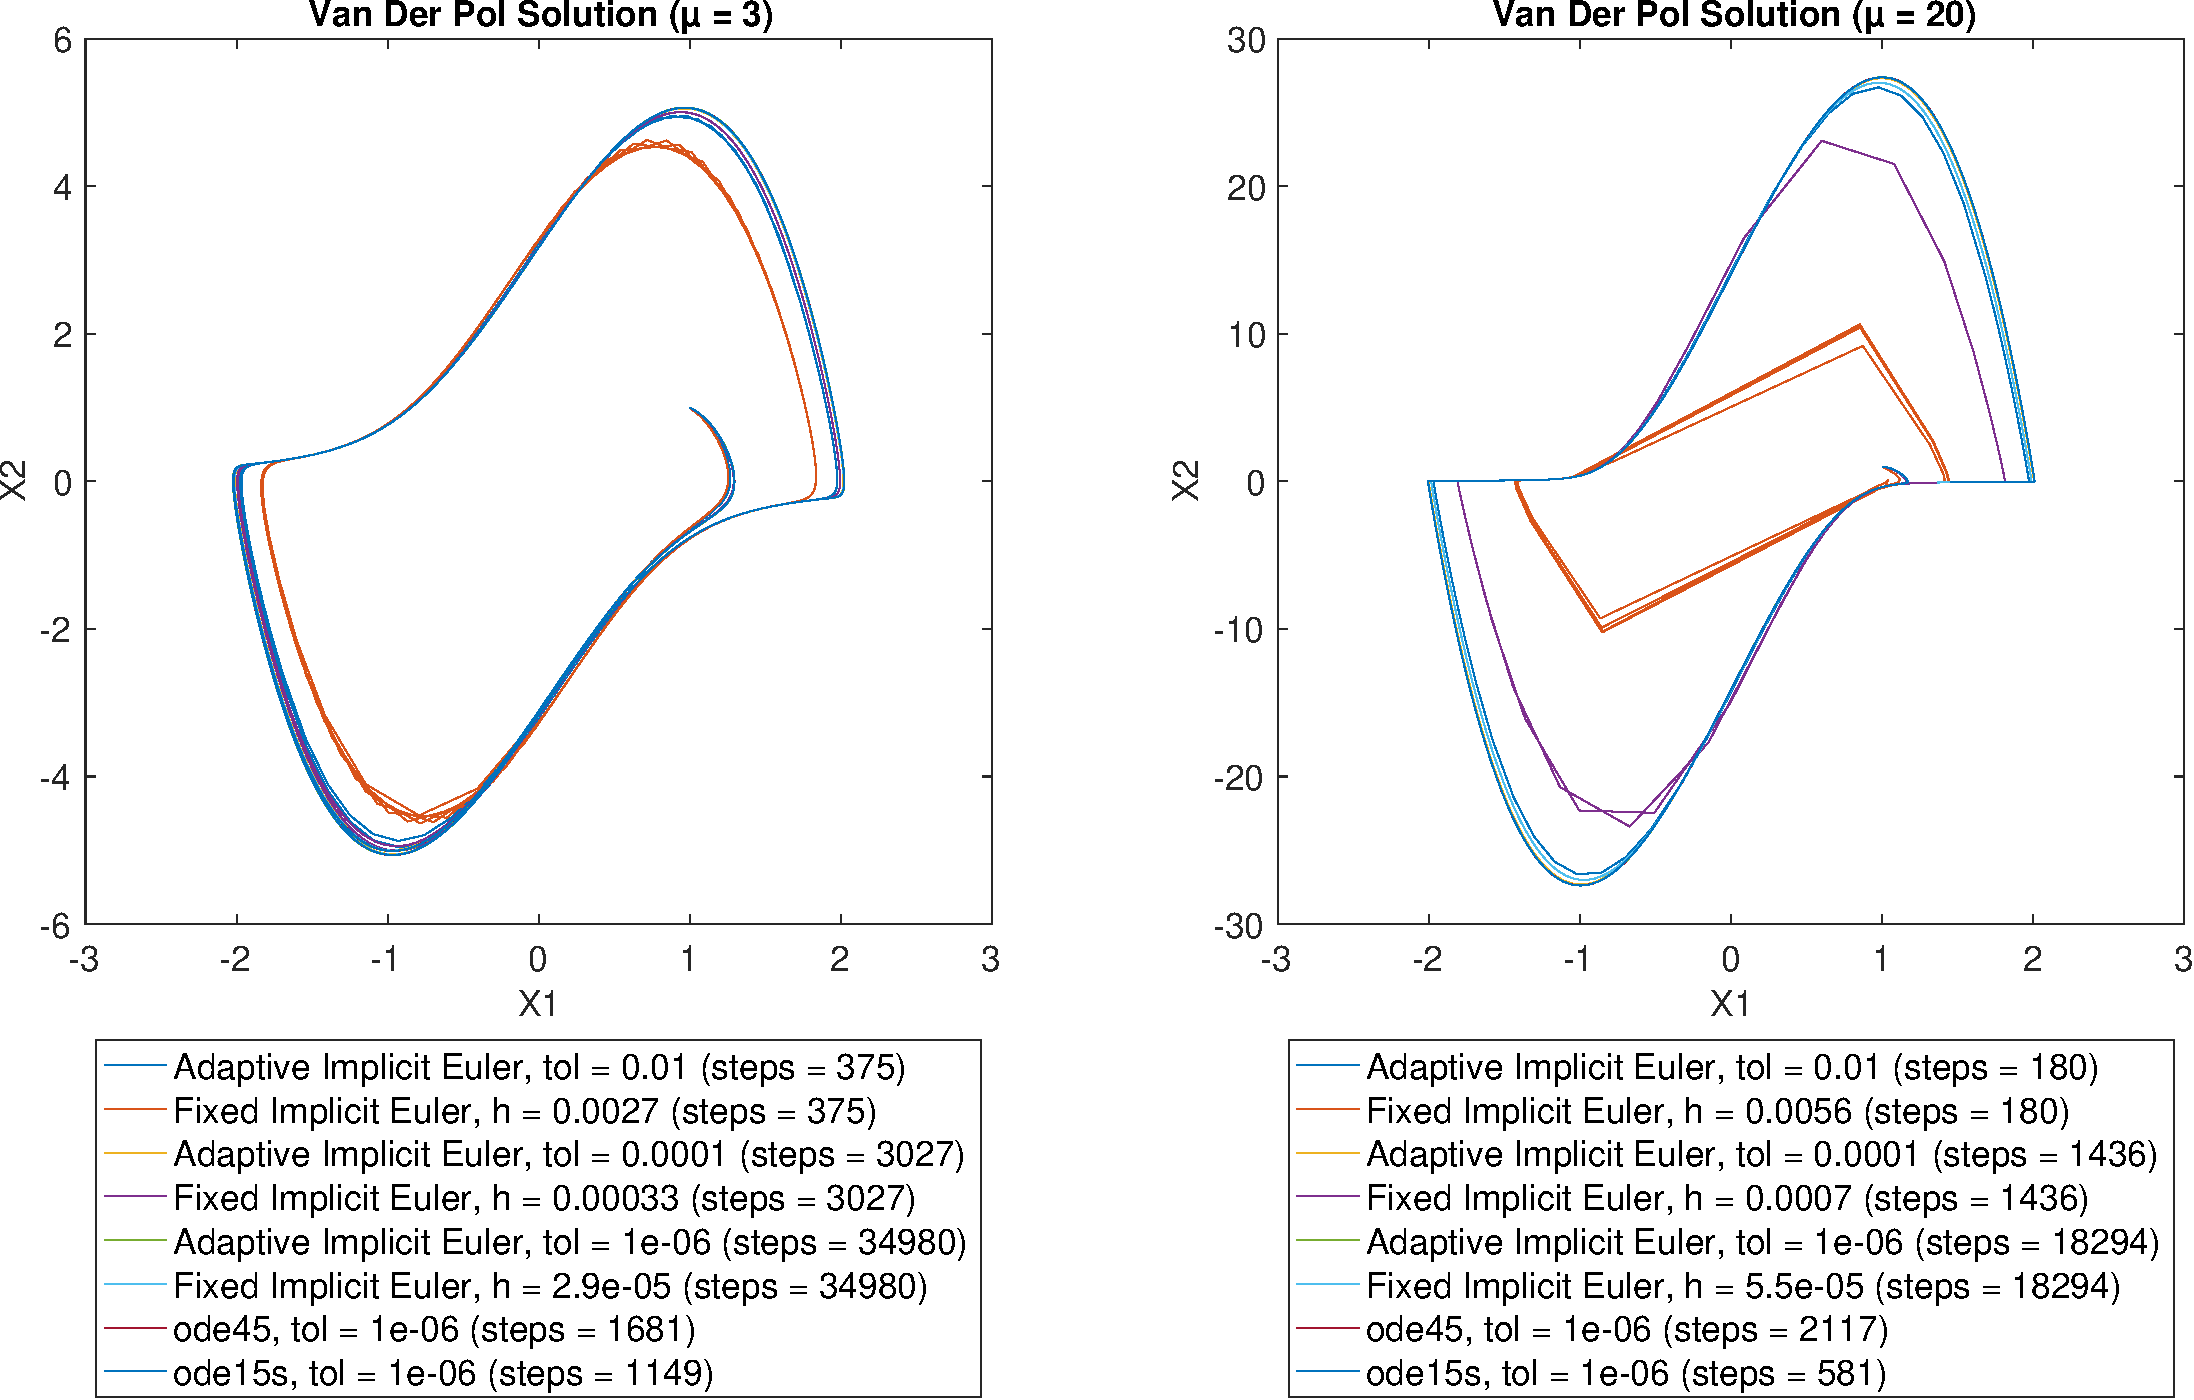
\includegraphics[width=\textwidth]{plots/3_4main.pdf}
    \caption{Implicit Euler method tested on the Van der Pol problem. Both an adaptive step size strategy with tolerance = 0.01 and a fixed step size strategy fixed to equal number of steps is applied.}
    \label{fig:2_4a}
\end{figure}


\subsection{Discussion of interface}
The methods have been implemented in a similar fashion to MATLAB's ode45 and ode15s for comparison purposes. For better comparison of fixed vs. adaptive step size, the implementation of the fixed step size was designed to be able to take a $N$ number of steps as input.